\datos{color}{}{}
\section*{Propuesta: optimización del \textit{rendezvous} para dos \textit{cobots} cooperativos}
\addcontentsline{toc}{section}{Propuesta: optimización del \textit{rendezvous} para dos \textit{cobots} cooperativos}

En el grupo de investigación en el que trabajo estamos comenzando un 
proyecto enmarcado en la agricultura vertical. En este sentido, estamos 
preparando un entorno, tanto real como simulado (Figura \ref{fig:sim}),
en el que dos robot manipuladores colaborativos van a desempeñar diferentes
tareas. Debido a que todavía estamos definiendo el escenario, lo más 
probable es que este varíe respecto de la imagen presentada, aunque
esas modificaciones no serán estructurales. Dos de los cambios incluyen 
que el robot de la izquierda tendrá también sus propias estanterías y que el 
robot de la derecha trabajará cerca 
de la pared cuando el eje lineal de desplazamiento sobre el que se coloca
esté en uno de sus extremos. \\

\begin{figure}[H]
  \centering
  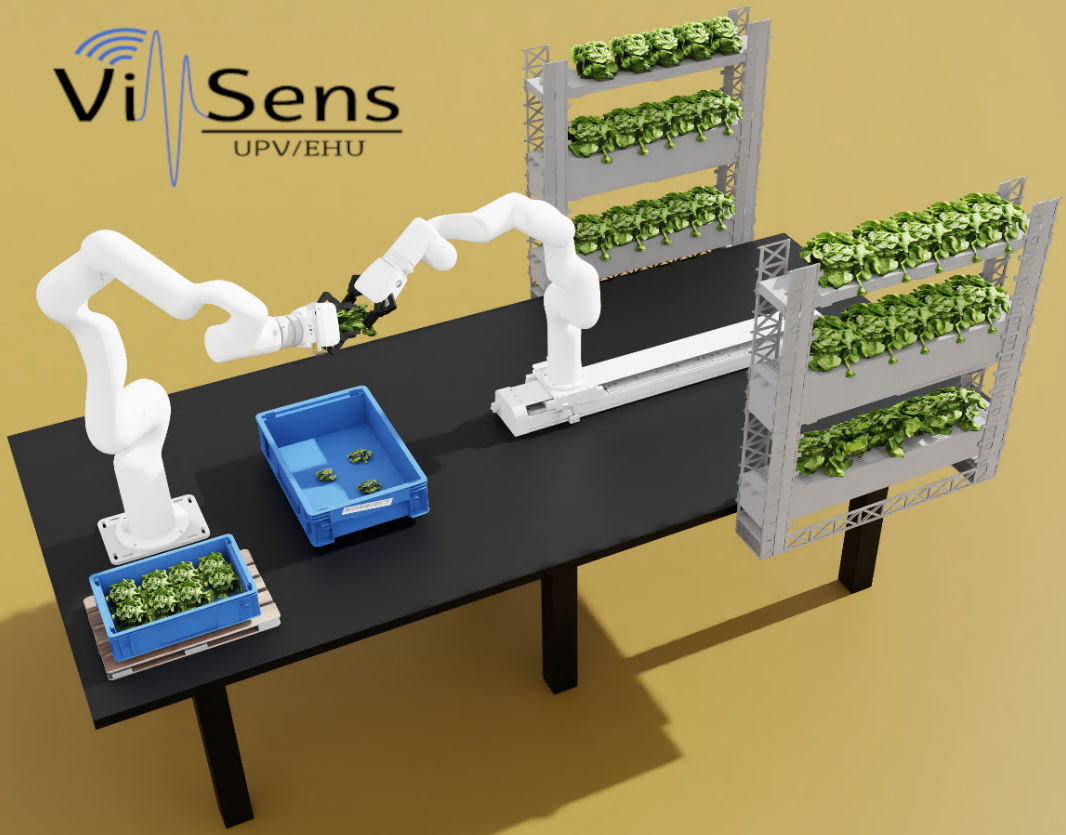
\includegraphics[scale=0.25]{Images/escenario3_visens.png}
  \caption{Escenario simulado.}
  \label{fig:sim}
\end{figure}

Este escenario está compuesto por una mesa, dos robots manipuladores 
colaborativos y estanterías de cultivo y almacenaje. La mesa es la superficie
sobre la que se desarrollará toda la actividad, por lo que los robots 
no deben exceder sus límites. El primer robot, el \textit{UFactory 850} \cite{ufactory_xarm850}, 
es el que está colocado a la izquierda en la Figura \ref{fig:sim}, y está
fijo a la mesa. El segundo robot, el \textit{UFactory xArm6} \cite{ufactory_xarm850}, es el que 
se encuentra a la derecha en la Figura \ref{fig:sim}, y está montado sobre un eje 
lineal de desplazamiento que le permite aumentar su espacio de trabajo.
Ambos robots están equipados con pinza, cámara de visión y sensor de fuerza 
en el efector. Las estanterías correspondientes a cada robot están colocadas de manera que son completamente 
alcanzables por los dos manipuladores. \\

El segundo robot se encargará de supervisar el estado de los cultivos o 
aplicarles alguna operación, 
y cuando considere necesario (bien sea por visión, o por tiempo de cultivo, por ejemplo)
retirará un cultivo para realizarle una operación o tratamiento que necesite 
de la cooperación con el primer robot, por ejemplo, la retirada de hojas enfermas.
En función del tratamiento aplicado, la hortaliza deberá volver a su 
estantería de cultivo, mediante el segundo robot, o ir a la estantería de almacenaje. 
En caso de ser almacenada,
será el primer robot el encargado de ejecutar dicha tarea. 
Por su parte, el primer robot traslada las hortalizas 
de la estantería de almacenaje a un palet o realiza alguna operación específica 
sobre las plantas en este momento del cultivo.\\

Además, en las tareas cooperativas será preciso controlar la fuerza aplicada 
por cada robot para evitar dañar las hortalizas, que se caracterizan 
por ser deformables. Siempre y cuando esta fuerza se controle adecuadamente 
por ambos robots, el punto de cooperación de los robots no tiene 
por qué ser fijo, esto es, en función de la situación instantánea de 
cada robot ese punto podrá darse en diferentes coordenadas, pero 
siempre garantizando que la fuerza aplicada a la planta es la adecuada. \\

%No obstante, por simplicidad este control de fuerzas podría quedar 
%fuera del problema de optimización. \\

Con todo ello, se busca un sistema autónomo y adaptativo en el que
los dos robots decidan en cada instante qué operación ejecutar
—retirar hojas, realizar tratamientos, regar, germinar o mover 
plantas al almacén, por ejemplo— de modo que el conjunto minimice el tiempo de
ciclo, o, en otras palabras, maximice la eficiencia operativa. \\

Como se ha explicado, este sistema está compuesto de múltiples partes,
pero esta propuesta de problema de optimización se va a centrar en el punto 
espacial de cooperación. A este punto se le denomina \textit{rendezvous}. 

\section*{Objetivo}
Obtener las posiciones, \(\mathbf{p}_r=(x_r,y_r,z_r)\), y orientaciones,
\(\mathbf{q}_r=(q_{r_0},q_{r_1},q_{r_2},q_{r_3})\), de los efectores de cada robot,
$r\in\{A,B\}$,
y los 
factores de velocidad de ejecución de movimiento de cada robot, \(\mathbf{s}_r\), incluyendo el 
del eje lineal de desplazamiento \(\mathbf{s}_{rail}\), que permitan
sincronizar la llegada de ambos robots al \textit{rendezvous} óptimo calculado ($p_r,\,q_r$) 
sincronizando y minimizando el 
tiempo de desplazamiento necesario, $t_{r}(\mathbf{p}_r,\mathbf{q}_r,\mathbf{s}_r)$,
según el estado actual de cada robot (posición actual). \\

Las posiciones se definen en el espacio de la tarea de cada robot y en metros, las 
orientaciones en cuaterniones, los factores de 
velocidad podrán tomar cualquier valor entre 0 y 1, y el tiempo de desplazamiento
se mide en segundos. La elección de cuaterniones para representar la orientación no es trivial,
dado que es la fórmula computacionalmente más 
eficiente \cite{barrientos2007fundamentos} al no presentar singularidades, ser más compactos y 
fáciles de normalizar.\\

Por tanto, se buscan las posiciones y orientaciones de los efectores 
\(\mathbf{p}_A=(x_A,y_A,z_A)\), \(\mathbf{p}_B=(x_B,y_B,z_B)\), 
\(\mathbf{q}_A=(q_{A_0},q_{A_1},q_{A_2},q_{A_3}),\, \mathbf{q}_B=(q_{B_0},q_{B_1},q_{B_2},q_{B_3})\), y los factores de velocidad de cada robot 
\(\mathbf{s}_A,\, \mathbf{s}_B,\, \mathbf{s}_{rail}\), tal que minimicen 
el tiempo de desplazamiento de cada robot al punto de cooperación,
$t_A(\mathbf{p}_A,\mathbf{q}_A,\mathbf{s}_A)$ y $\,t_B(\mathbf{p}_B,\mathbf{q}_B,\mathbf{s}_B,\mathbf{s}_{rail})$, 
y ambos sean lo más parecidos posible. \\

Es decir, ambos robots deben llegar sincronizados al \textit{rendezvous}.Es importante mencionar que,
puesto que el segundo robot $B$ está sobre un eje lineal de desplazamiento, su tiempo $t_B$ tiene que
tener en cuenta también el factor de velocidad de dicho eje, $s_{rail}$. \\

En el punto de cooperación o \textit{rendezvous} los efectores deben quedar enfrentados,
esto es, alineados en dos ejes del mundo y separados por una determinada distancia en el otro. 
Esta configuración, Figura \ref{fig:conf}, implica que la diferencia en la orientación
en ambos será de 180º y la distancia se medirá en línea recta desde los orígenes
de ambos efectores, para lo que será necesario convertir las posiciones $p_A$ y $p_B$
a coordenadas del mundo.

\begin{figure}[H]
  \centering
  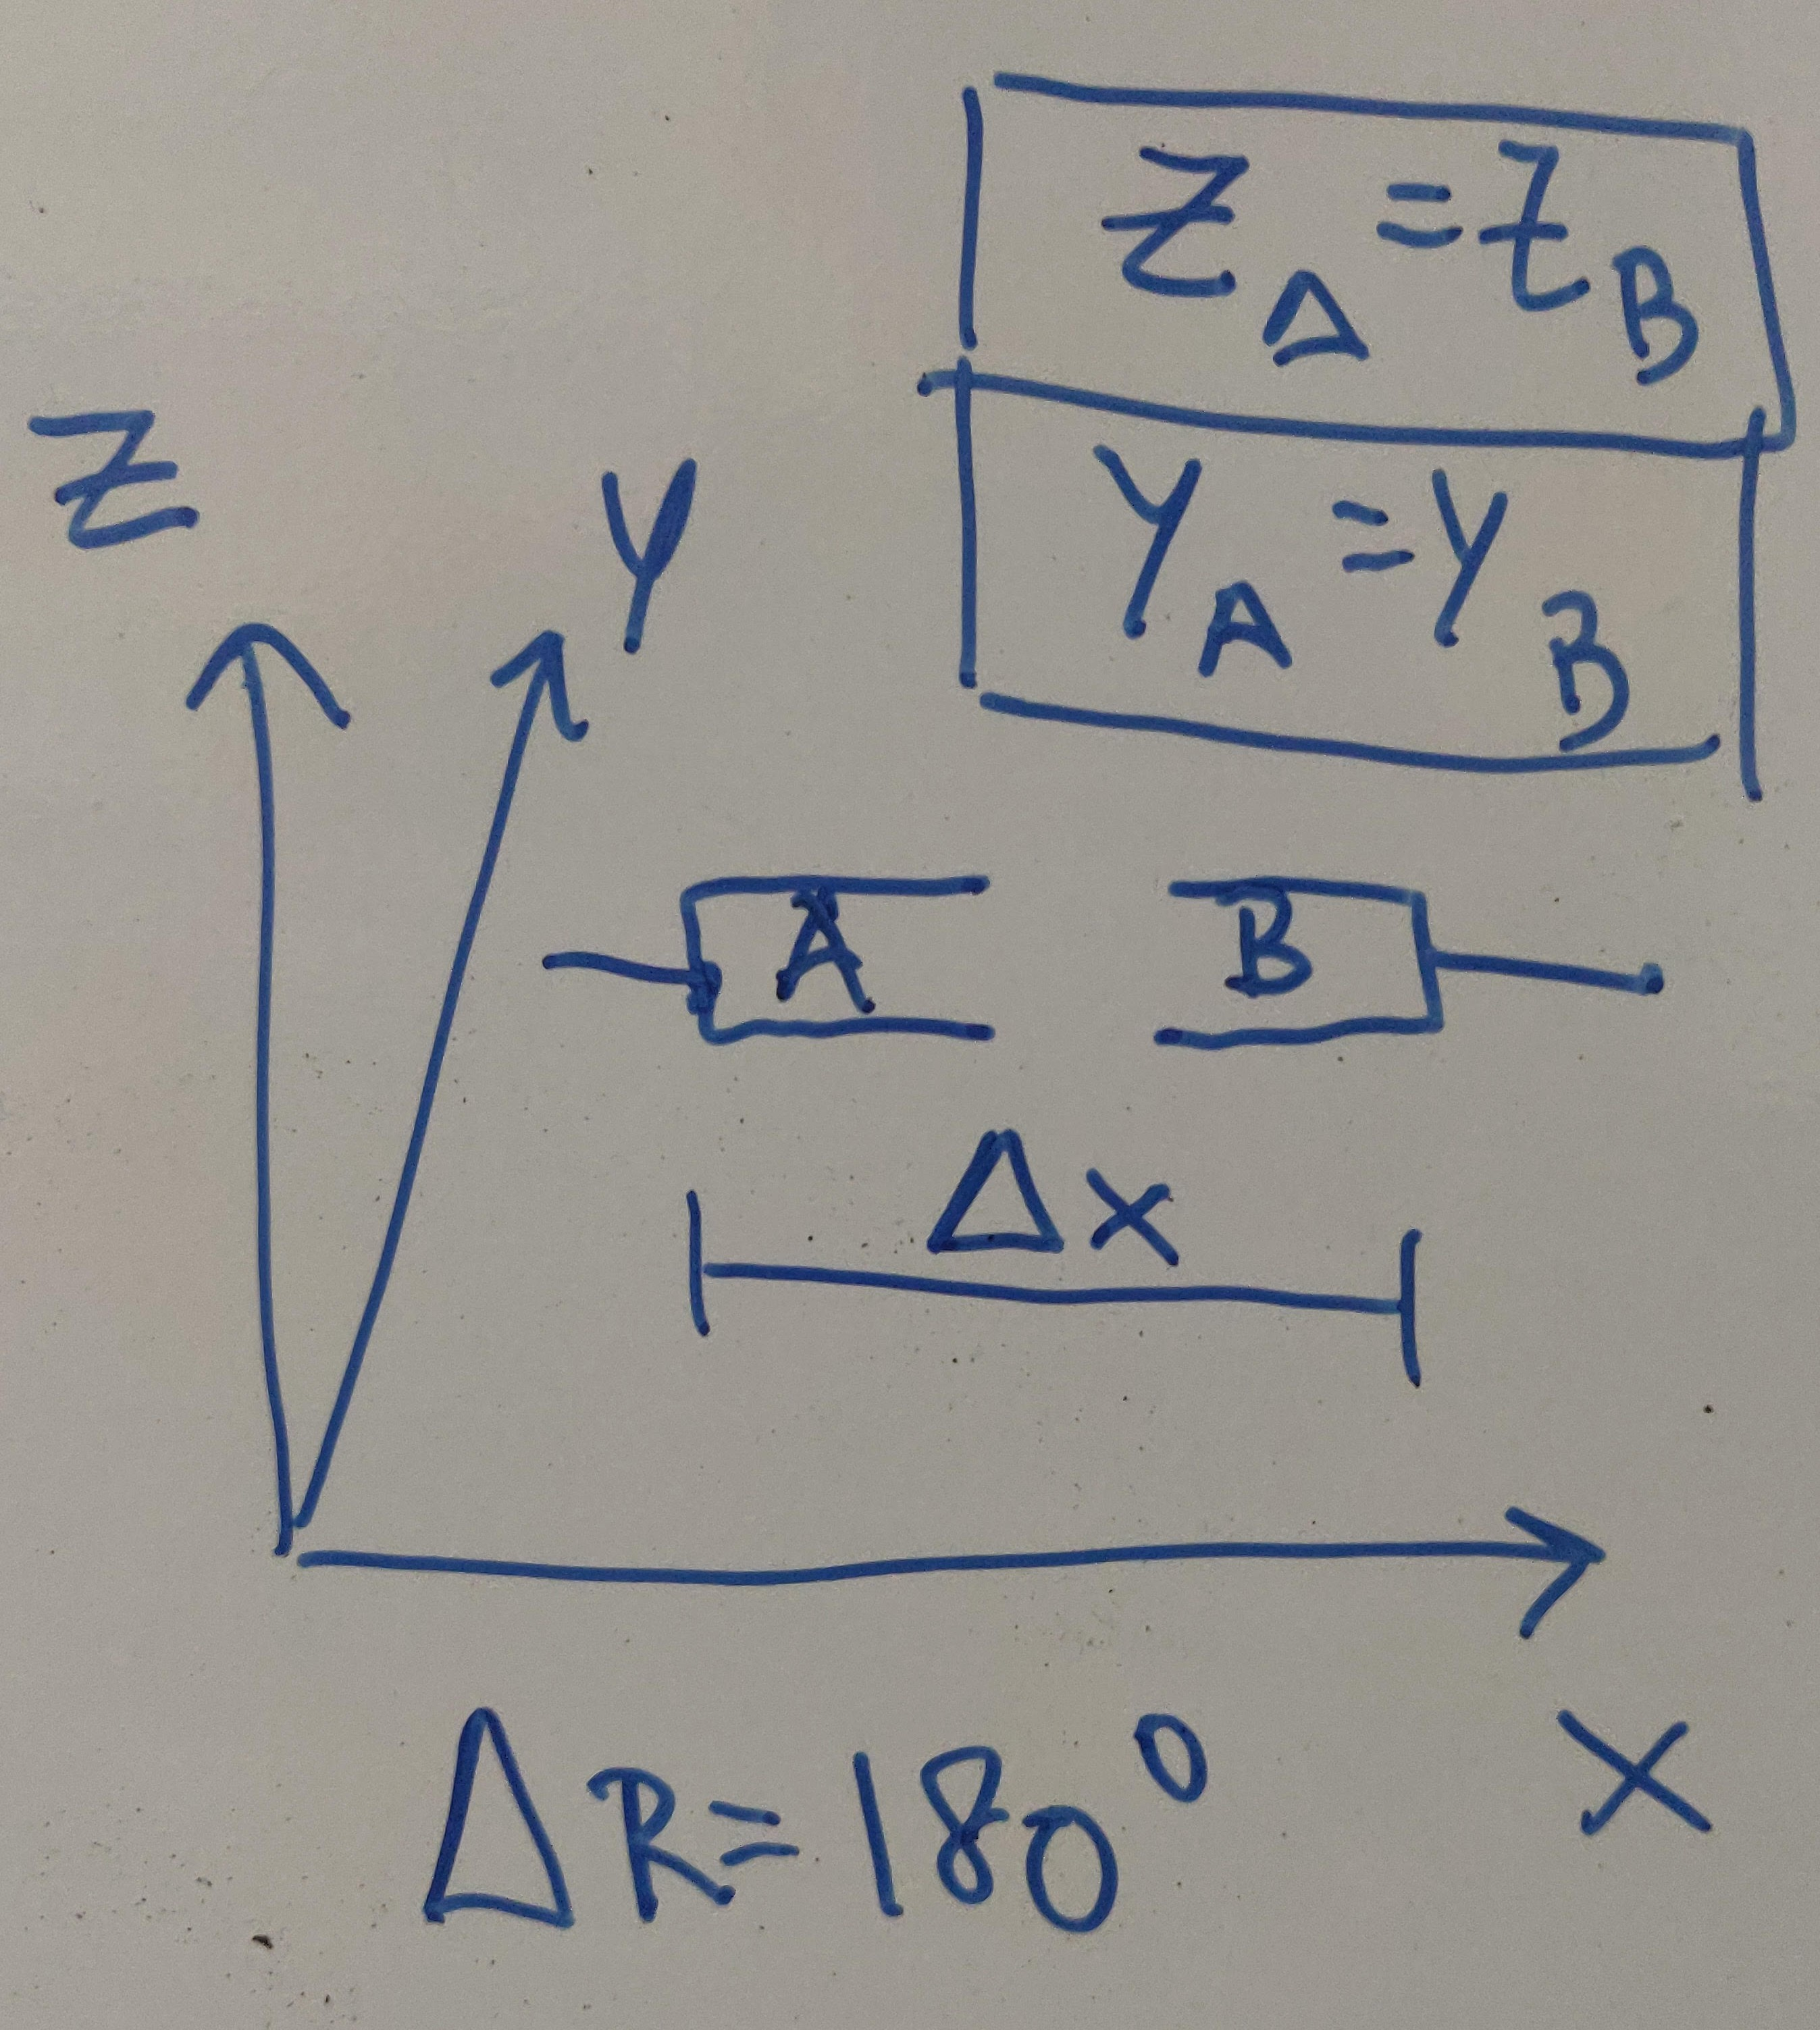
\includegraphics[scale=0.05]{Images/ejemplo.jpg}
  \caption{Croquis de la configuración propuesta.}
  \label{fig:conf}
\end{figure}

En otras palabras, el objetivo es obtener las coordenadas óptimas del punto de cooperación \textit{rendezvous}
y los factores de velocidad de cada robot de manera que se minimice el tiempo de llegada 
sincronizada al mismo.


\section*{Variables de decisión}
\addcontentsline{toc}{subsection}{Variables de decisión}
Se tiene un total de 17 variables de decisión:
\begin{itemize}
  \item \textbf{Posiciones objetivo de efectores}: \(\mathbf{p}_A=(x_A,y_A,z_A)\), \(\mathbf{p}_B=(x_B,y_B,z_B)\) 
  en el espacio de la tarea de cada robot.
  \item \textbf{Orientaciones objetivo de efectores}: 
  \(\mathbf{q}_A,\, \mathbf{q}_B \in S^3,\) donde cada cuaternión unitario $\mathbf{q}=(q_{0},q_{1},q_{2},q_{3})$ representa una rotación en $SO(3)$.
  %\(\mathbf{R}_A,\mathbf{R}_B\in SO(3)\).
  \item \textbf{Escalas de velocidad}: \(\mathbf{s}_A,\mathbf{s}_B, \mathbf{s}_{rail}\in(0,1]\).
\end{itemize}

\begin{comment}
\subsection*{Parámetros y variables derivadas}
\addcontentsline{toc}{subsection}{Parámetros y variables derivadas}

\begin{itemize}
  \item \textbf{Variables derivadas}: \(t_A,t_B\) tiempos estimados de llegada, calculados mediante la función de tiempo
  

\[
  t_r(\mathbf{p}_r,\mathbf{R}_r,s_r),
  \]


  y no tratadas como variables independientes en la optimización.
  \item \textbf{Parámetros del problema}: \(d_{\text{ef}}\) (distancia objetivo entre efectores), \(\text{eje}\in\{x,y\}\) (eje del mundo para la separación), \(\epsilon\) (tolerancia posicional), \(\Delta t_{\max}\) (tolerancia temporal de sincronización), \(s_{\min}\), \(m_{\min}\), y otros límites físicos.
\end{itemize}
\end{comment}

\section*{Función objetivo}
\addcontentsline{toc}{subsection}{Función objetivo}
\[
\min_{\mathbf{p}_A,\mathbf{q}_A,\mathbf{p}_B,\mathbf{q}_B,\mathbf{s}_A,\mathbf{s}_B,\mathbf{s}_{rail}}\; 
T_{\text{rendezvous}} \;=\; \min\; \max\big(t_A(\mathbf{p}_A,\mathbf{q}_A,\mathbf{s}_A),\,t_B(\mathbf{p}_B,\mathbf{q}_B,\mathbf{s}_B,\mathbf{s}_{rail})\big),
\]

donde los tiempos $t_A$ y $t_B$ se refiere a los tiempos $t_{r}(\mathbf{p}_r,\mathbf{q}_r,\mathbf{s}_r)$
necesarios por cada robot para alcanzar
el punto de cooperación. Se estima de la siguiente manera:
\[
t_{r}(\mathbf{p}_r,\mathbf{q}_r,\mathbf{s}_r)
=\frac{\text{dist\_rail}(\mathbf{p}_r)}{s_{rail}\,v_{\text{rail}}}
+\frac{\ell_r(\mathbf{p}_r,\mathbf{q}_r)}{s_r\,v_{\text{arm},r}},
\]

%donde \(\ell_r\) aproxima la distancia efectiva necesaria para alcanzar posición y orientación.\\

En esta expresión \(\mathrm{dist\_rail}(\mathbf{p}_r)\) es la distancia a recorrer 
por el motor lineal (raíl) en metros (si no existe raíl, es decir, el robot 
está fijo -robot A-, se toma \(0\)),
\(v_{\text{rail}}\) es la velocidad del raíl en \(\mathrm{m/s}\), 
\(\ell_r(\mathbf{p}_r,\mathbf{R}_r)\) es la longitud
efectiva del movimiento del brazo en metros (por ejemplo, la distancia euclídea del efector
desde su posición inicial con todas las articulaciones en posición $0$), y \(v_{\text{arm},r}\) es la 
velocidad del brazo en \(\mathrm{m/s}\). Dividir por \(s_r\)
reduce la velocidad efectiva y por tanto, aumenta el tiempo. \\

Cabe mencionar que la primera evaluación del equipo docente valoró la sustitución de la función
$\min\; \max (·)$ por un frente de pareto multiobjetivo con dos funciones objetivo, una por cada robot:

\[
\min_{\mathbf{p}_A,\mathbf{q}_A,\mathbf{p}_B,\mathbf{q}_B,\mathbf{s}_A,\mathbf{s}_B,\mathbf{s}_{rail}}
\;\; \mathbf{T}(\cdot),
\]

con
\[
\mathbf{T}(\cdot) = 
\begin{bmatrix}
t_A(\mathbf{p}_A,\mathbf{q}_A,\mathbf{s}_A) \\
t_B(\mathbf{p}_B,\mathbf{q}_B,\mathbf{s}_B,\mathbf{s}_{rail})
\end{bmatrix},
\]

Así, una solución $\mathbf{x}^\star$ se considera óptima en el sentido de Pareto si no 
existe otra solución factible $\mathbf{x}$ tal que
\[
t_A(\mathbf{x}) \le t_A(\mathbf{x}^\star), \qquad
t_B(\mathbf{x}) \le t_B(\mathbf{x}^\star),
\]

y al menos una de las desigualdades sea estricta ($<$). El conjunto de todas las soluciones 
Pareto-óptimas constituye el frente de Pareto en el plano $(t_A,t_B)$, que describe 
los compromisos entre minimizar el tiempo de llegada del robot A y el del robot B. \\

Mientras que con Pareto no hay una única solución y se necesitaría
un criterio externo para elegir un punto de entre los Pareto-óptimos,
la formulación con $\min\; \max (·)$ obtiene una única solución. Puesto que se 
desea que ambos robots lleguen sincronizados, en otras palabras, que tarden lo mismo, 
se va a optar por $\min\; \max (·)$, aunque se deja la puerta abierta a 
resolver también el problema como frente de Pareto y así desarrollar una comparativa.


\section*{Restricciones}
\addcontentsline{toc}{subsection}{Restricciones}
\begin{itemize}
  \item Separación final en coordenadas del mundo. Los efectores deben quedar separados 
  por la distancia objetivo \(d_{\text{ef}}\) en el eje asignado, cuyo eje unitario se representa mediante 
  $\mathbf{e}_{\text{eje}}^\top$, y con tolerancia \(\epsilon_{\text{eje}}\):
  $
  \big|\mathbf{e}_{\text{eje}}^\top\big((\mathbf{p}_A)-(\mathbf{p}_B)\big)-d_{\text{ef}}\big|\le\epsilon_{\text{eje}}
  $.

  \item Posición y orientación de enfrentamiento: \textit{rendezvous} enfrentado. 
  Siguiendo la representación de la Figura \ref{fig:conf}:\\
  \[\big|\mathbf{e}_{\text{Z}}^\top\big((\mathbf{p}_A)-(\mathbf{p}_B)\big)|\le\epsilon_Z, 
  \qquad\big|\mathbf{e}_{\text{Y}}^\top\big((\mathbf{p}_A)-(\mathbf{p}_B)\big)|\le\epsilon_Y\]
  \[
  \|\operatorname{Log}(\mathbf{R}_B \mathbf{R}_A^\top \mathbf{R}_{\pi}^\top)\|\le \epsilon_{\theta},
  \]

  %donde \(\mathbf{R}_{\pi}\) es la rotación de 180° que define la orientación volteada y \(\operatorname{Log}(\cdot)\)
  %es el mapa logaritmo de rotaciones (norma en radianes).
  %, que convierte una matriz de rotación
  %en su representación eje-ángulo, de modo que la norma del resultado mide directamente el
  %ángulo mínimo de rotación necesario para ir de una orientación a otra. 
  %Por eso se usa en la desigualdad, ya que cuantifica la desviación angular (en radianes) 
  %respecto a la orientación volteada (\url{https://cvg.cit.tum.de/_media/members/demmeln/nurlanov2021so3log.pdf},
  %\url{https://colab.research.google.com/github/borglab/gtsam/blob/develop/gtsam/geometry/doc/SO3.ipynb}). \\


  donde \(\mathbf{R}_{\pi}\) es la rotación de 180° que define la orientación volteada y \(\operatorname{Log}(\cdot)\)
  es el mapa logaritmo de rotaciones (norma en radianes). \\

  Aunque las orientaciones se parametrizan mediante cuaterniones en las variables de decisión, 
  para evaluar las restricciones resulta conveniente convertirlos a matrices de rotación $\mathbf{R}_r$. La 
  representación en $SO(3)$ permite operar directamente con la composición de rotaciones y, 
  en particular, aplicar el mapa logarítmico $\operatorname{Log}(\cdot)$, que transforma una 
  matriz de rotación en su representación eje–ángulo \cite{murray1994mathematical}. La norma de este vector proporciona una 
  medida angular interpretable y numéricamente estable del error entre orientaciones, equivalente
  al ángulo mínimo necesario para alinear una con la otra \cite{barfoot2014associating}. Por ello, la restricción 
  $\|\operatorname{Log}(\mathbf{R}_B \mathbf{R}_A^\top \mathbf{R}_{\pi}^\top)\|\le \epsilon_{\theta}$ 
  cuantifica de manera directa la desviación respecto a la orientación enfrentada deseada. De este
  modo, las restricciones de alineación y enfrentamiento pueden formularse de forma más natural y
  robusta, manteniendo al mismo tiempo la compacidad y suavidad de los cuaterniones como 
  parametrización principal en la optimización (\url{https://cvg.cit.tum.de/_media/members/demmeln/nurlanov2021so3log.pdf},
  \url{https://colab.research.google.com/github/borglab/gtsam/blob/develop/gtsam/geometry/doc/SO3.ipynb}). \\


  
  %Aunque las orientaciones se parametrizan mediante cuaterniones en las variables de decisión, 
  %para la formulación de las restricciones resulta conveniente convertirlos
  %a matrices de rotación. Esta representación en $SO(3)$ permite expresar de forma directa operaciones
  %geométricas como la composición de rotaciones, el cálculo del error relativo entre orientaciones o 
  %la aplicación del mapa logarítmico, cuya norma proporciona una medida angular interpretable y 
  %numéricamente estable. De este modo, las restricciones de enfrentamiento y alineación pueden 
  %formularse de manera más natural y robusta, manteniendo al mismo tiempo la compacidad y suavidad
  %de los cuaterniones como variables de decisión.

  Esta restricción, aparentemente dura, se ha diseñado como blanda puesto que el objetivo a largo
  plazo será que el \textit{rendezvous} se pueda alcanzar con diferentes orientaciones y alineaciones.
  No obstante, para simplificar el proyecto dentro de la asignatura, se instroduce la restricción.
  %Para formulaciones con cuaterniones:
  %\[
  %q_B \approx q_{\pi}\otimes q_A,\qquad
  %\arccos\big(|\langle q_B,\,q_{\pi}\otimes q_A\rangle|\big)\le \epsilon_{\theta}.
  %\]

  %Elige \(\epsilon_{\perp}\) pequeño (p. ej. \(10^{-3}\)) y \(\epsilon_{\theta}\) en radianes (p. ej. \(0.01\)–\(0.05\)) según tolerancias de la tarea.


%\[
%\mathbf{R}_B = \mathbf{R}_{\pi}\,\mathbf{R}_A
%\qquad\Longleftrightarrow\qquad
%\mathbf{R}_B\,\mathbf{R}_A^\top = \mathbf{R}_{\pi}.
%\]

%\[
%\mathbf{R}_B = \mathbf{R}_A\,\mathbf{R}_{\pi}^{\text{(tool)}},
%\]

%\[
%\mathbf{R}_{\pi}=\exp\big(\pi\,[\mathbf{u}]_\times\big)
%= I + 2\big(\mathbf{u}\mathbf{u}^\top - I\big),
%\]





  \item Sincronización temporal. Llegadas casi simultáneas dentro de la tolerancia \(\Delta t_{\max}\):
  $\big|t_A(\mathbf{p}_A,\mathbf{q}_A,\mathbf{s}_A)-t_B(\mathbf{p}_B,\mathbf{q}_B,\mathbf{s}_B,\mathbf{s}_{rail})\big| \le \Delta t_{\max}$.

  \item Límites de escala de velocidad: 
  $0 < s_A \le 1,\quad 0 < s_B \le 1,$
  siendo $1$ la velocidad máxima permitida por el robot. Esta restricción será por definición 
  del problema y no una restricción pura a validar por el algoritmo.

  \item Exclusión de singularidades y factibilidad cinemática.
  Para cada pose y orientación objetivo debe existir una solución de cinemática 
  inversa \(q_r\) alcanzable:

  $\exists q_r:\ FK_r(q_r)=(\mathbf{p}_r,\mathbf{R}_r),\qquad
  \sigma_{\min}\big(J_r(q_r)\big)\ge m_{\min}$,
  donde $\sigma_{\min}\big(J_r(q_r)\big)$ es el menor valor singular de la jacobiana en 
  $q_r$, es decir, una medida numérica de cuán cerca está la configuración de una singularidad.
  Valores pequeños indican pérdida de grado de libertad efectivo, es decir, que se 
  encuentra cerca de una singularidad. Si existen múltiples soluciones \textit{IK}
  (cinemática inversa), se selecciona la que maximice \(\sigma_{\min}\).

  \item Espacio de trabajo $\mathcal{W}_r$ y zonas prohibidas $\mathcal{Z}_{r}$ de 
  cada robot $r$.
  Las poses deben pertenecer al espacio de trabajo y evitar zonas prohibidas:
  $
  (\mathbf{p}_r,\mathbf{R}_r)\in\mathcal{W}_r\setminus\mathcal{Z}_{r},\qquad r\in\{A,B\}.
  $ Esta restricción debería ser dura porque si no se cumple la solución es directamente 
  no factible. No obstante, esta restricción también irá ligada a la definición 
  del problema y no será una restricción pura a validar por el algoritmo.

\end{itemize}

\begin{comment}
Denotando \(\operatorname{proj}_{\text{eje}}(\mathbf{p})\) la proyección de la coordenada 
correspondiente al eje del mundo:

\[
\begin{cases}
\text{si eje}=x:\quad |(x_A-x_B)-d_{\text{ef}}|\le \epsilon,\\
\text{si eje}=y:\quad |(y_A-y_B)-d_{\text{ef}}|\le \epsilon.
\end{cases}
\]
\end{comment}


\section*{Función de mérito penalizada}
\addcontentsline{toc}{subsection}{Función de mérito penalizada}
En primera instancia se propuso una función de mérito que combinaba el objetivo principal, 
$T_{\max}(\cdot)=\max\big(t_A(\cdot),t_B(\cdot)\big)$, donde \(\cdot\) 
denota el conjunto de variables de decisión, con las siguientes penalizaciones
por violación de restricciones blandas:

\begin{itemize}
  \item \textbf{Penalización de separación:} penaliza desviaciones mayores que \(\epsilon\)
  respecto a la distancia objetivo \(d_{\text{ef}}\) proyectada sobre el eje.
\[
  P_{\text{sep}}(\mathbf{p}_A,\mathbf{p}_B)
  =\Big(\max\big(0,\;|\operatorname{proj}_{\text{eje}}(\mathbf{p}_A)-\operatorname{proj}_{\text{eje}}(\mathbf{p}_B)-d_{\text{ef}}|- \epsilon\big)\Big)^2,
  \]

  \item \textbf{Penalización de alineación:} penaliza desviaciones en la alineación de 
  los efectores en el \textit{rendezvous}.
\[
\begin{aligned}
P_{\text{alineación}}(\mathbf{p}_A,\mathbf{p}_B,\mathbf{R}_A,\mathbf{R}_B)
&= \big(\max\big(0,\;|\mathbf{e}_Z^\top(\mathbf{p}_A-\mathbf{p}_B)|-\epsilon_Z\big)\big)^2 \\
&\quad + \big(\max\big(0,\;|\mathbf{e}_Y^\top(\mathbf{p}_A-\mathbf{p}_B)|-\epsilon_Y\big)\big)^2 \\
&\quad + \big(\max\big(0,\;\|\operatorname{Log}(\mathbf{R}_B\mathbf{R}_A^\top\mathbf{R}_{\pi}^\top)\|-\epsilon_{\theta}\big)\big)^2.
\end{aligned}
\]

  \item \textbf{Penalización de sincronización:} penaliza desincronizaciones mayores que la tolerancia \(\Delta t_{\max}\).
\[
  P_{\text{sync}}(t_A,t_B)
  =\Big(\max\big(0,\;|t_A-t_B|-\Delta t_{\max}\big)\Big)^2,
  \]
  

  \item \textbf{Penalización de singularidades:} penaliza configuraciones con manipulabilidad por debajo del umbral \(m_{\min}\); \(\sigma_{\min}(J_r)\) es el menor valor singular del Jacobiano.
\[
  P_{\text{sing}}(\mathbf{p}_r,\mathbf{R}_r)
  =\sum_{r\in\{A,B\}} \Big(\max\big(0,\;m_{\min}-\sigma_{\min}(J_r(q_r(\mathbf{p}_r,\mathbf{R}_r)))\big)\Big)^2,
  \]

\end{itemize}
Las penalizaciones se definen como cuadráticas porque castigan más fuertemente 
las violaciones grandes que las pequeñas, lo que incentiva al optimizador a priorizar
correcciones moderadas antes que soluciones extremas. \\

La función de mérito quedaba de la siguiente manera:
\[
  J_{\text{total}}(\cdot)
  = T_{\max}(\cdot)
  + P_{\text{sep}}(\mathbf{p}_A,\mathbf{p}_B)
  + P_{\text{alineación}}(\mathbf{p}_A,\mathbf{p}_B,\mathbf{R}_A,\mathbf{R}_B)
  + P_{\text{sync}}(t_A,t_B)
  + P_{\text{sing}}(\mathbf{p}_r,\mathbf{R}_r).
\]

Sin embargo, tras la primera evaluación del equipo docente se ha decidido suprimir la 
presencia de la función objetivo en la función de mérito. Esto se debe a que sería necesario 
introducir ponderaciones de difícil sintonización con el riesgo de introducir posibles 
discontinuidades asociadas al operador $max(⋅)$. \\

Se va a ilustrar mediante un ejemplo. Sean dos soluciones distintas para las variables de decisión donde
la primera conlleva un menor tiempo de desplazamiento, pero no es tan precisa como la segunda. 
En estos casos, puede que nos interese más la segunda solución, pero introducir la función 
objetivo en la de mérito podría provocar que se desechara. \\

Consecuentemente, la función de mérito propuesta es la siguiente: 
\[
  J_{\text{total}}(\cdot)
  = P_{\text{sep}}(\mathbf{p}_A,\mathbf{p}_B)
  + P_{\text{alineación}}(\mathbf{p}_A,\mathbf{p}_B,\mathbf{R}_A,\mathbf{R}_B)
  + P_{\text{sync}}(t_A,t_B)
  + P_{\text{sing}}(\mathbf{p}_r,\mathbf{R}_r).
\]

\begin{comment}
  \[
  J_{\text{total}}(\cdot)
  = T_{\max}(\cdot)
  + \lambda_{\text{sep}}\,P_{\text{sep}}(\mathbf{p}_A,\mathbf{p}_B)
  + \lambda_{\text{sync}}\,P_{\text{sync}}(t_A,t_B)
  + \lambda_{\text{sing}}\,P_{\text{sing}}(\mathbf{p}_r,\mathbf{R}_r)
  + \lambda_{\text{ws}}\,P_{\text{ws}}(\mathbf{p}_r,\mathbf{R}_r),
\]

con \(\lambda_{\text{sep}},\lambda_{\text{sync}},\lambda_{\text{sing}},\lambda_{\text{ws}}\ge 0\) (pesos que ajustan la importancia relativa de cada penalización).
\end{comment}


\section*{Notas}
\addcontentsline{toc}{subsection}{Notas}
La restricción sobre la exclusión de singularidades puede omitirse en una primera fase para 
simplificar el problema, y una vez resuelto, añadirla para ampliar el problema de manera 
escalonada. \\

Las restricciones de los factores de velocidad y de los espacios de trabajo se establecen como
definición del problema. De esta manera, el algoritmo siempre generará nuevas soluciones 
dentro de las cotas establecidas en la naturaleza del problema. Por ejemplo, resulta evidente 
que las velocidades solo podrán estar en el rango $[0,\, 100] \%$. Por tanto, no se le permite generar
una solución con un valor fuera de ese rango facilitando así la búsqueda de soluciones. \\

%La restricción sobre el espacio de trabajo es dura, puesto que si los puntos calculados 
%están fuera del alcance de los robots, no serán factible. \\

Todas las restricciones posicionales y orientacionales se evalúan en coordenadas del mundo:
las poses objetivo se transforman desde la base del robot al mundo antes de aplicar las 
desigualdades anteriores. \\

La verificación de colisiones entre los robots durante las trayectorias que les permiten 
desplazarse desde la posición y orientación actual al \textit{rendezvous} óptimo calculado 
queda fuera del alcance de este problema de optimización. Esto se debe a que se 
considera un problema del nivel de la planificación de trayectorias. \\

La principal línea de trabajo del problema es su resolución mediante la función objetivo
$\min\; \max (·)$. Asimismo, se contempla la posibilidad de abordar el problema desde 
una perspectiva multiobjetivo, obteniendo el correspondiente frente de Pareto, para realizar
una comparativa entre ambos diseños.